\documentclass[10pt,a4paper]{scrartcl}
\usepackage[utf8x]{inputenc}
\usepackage[english,german]{babel}
\usepackage{amsmath}
\usepackage{amssymb}
\usepackage{graphicx}
\usepackage{listings}
\usepackage[format=plain,indention=1cm,font=sf ,labelfont=bf, nooneline,center]{caption}
\renewcommand{\captionfont}{\sffamily \slshape}
\renewcommand{\captionlabelfont}{ \sffamily \slshape \bfseries   }
\usepackage{subcaption}
\usepackage{url}
\usepackage{empheq}
\usepackage{dcolumn}
\usepackage{rotating}
\newcolumntype{d}{D{.}{.}{-1} }

\usepackage{tikz}
% \usetikzlibrary{circuits.ee.IEC,matrix,
% circuits.logic.US,
% circuits.logic.IEC,
% circuits.logic.CDH}
\usepackage{circuitikz}

% Quelle https://trucastuces.wordpress.com/2012/10/10/boxed-equations-in-latex/
\newlength\dlf  % Define a new measure, dlf
\newcommand\alignedbox[2]{
    % Argument #1 = before & if there were no box (lhs)
        % Argument #2 = after & if there were no box (rhs)
        &  % Alignment sign of the line
        {
            \settowidth\dlf{$\displaystyle #1$}
            % The width of \dlf is the width of the lhs, with a displaystyle font
                \addtolength\dlf{\fboxsep+\fboxrule}
            % Add to it the distance to the box, and the width of the line of the box
                \hspace{-\dlf}
            % Move everything dlf units to the left, so that & #1 #2 is aligned under #1 & #2
                \boxed{#1 #2}
            % Put a box around lhs and rhs
        }
}

\newcommand{\myscope}[2] % #1 = name , #2 = rotation angle
{\draw[thick,rotate=#2] (#1) circle (12pt)
    (#1) ++(-0.35,-0.1) -- ++(0.3,0.3) --++(0,-0.3)-- ++(0.3,0.3) --++(0,-0.3);
}

\title {Physikalisches Fortgeschrittenenpraktikum I\linebreak
Halbleiterbauelemente}
\author {\emph{Clemens Kurzenberg}\\212204196}
\date {30.04.2015}

\begin{document}

\maketitle

\begin{abstract}
    Im Rahmen dieses Versuches werden die wichtigsten Eigenschaften eines
    Operationsverstärkers vermessen,
    namentlich Offsetspannung, Eingangsruhestrom, Leerlaufverstärkung,
    Phasenverschiebung und Gleichtaktunterdrückung.
    Außerdem werden je ein Invertierender und Nichtinvertierender Verstärker,
    sowie ein Strom-Spannungswandler untersucht.
\end{abstract}

\tableofcontents

\pagebreak
\listoffigures
\listoftables

\pagebreak
\section {Einführung}

% TODO: verwendete Geräte

Operationsverstärker sind komplexe elektronische Bauelemente,
deren Zweck es ist, ein Signal zu verstärken.
Dies geschieht durch anlegen einer externen Gleichspannung
(Gleichtaktverstärkung)
mithilfe zahlreicher interner Halbleiterbauelemente.
Die erste Phase ist hierbei ein Differenzenverstärker,
der dafür sorgt,
dass an beiden Eingängen des Operationsverstärkers die gleiche Spannung anliegt.
Diese Eigenschaft ist essenziell bei der Herleitung des Übertragungsverhaltens
einer Schaltung,
die einen Operationsverstärker beinhaltet.
% TODO: Skizze?

Die Eigenschaften für einen idealen und einen realen Operationsverstärker
sind in Tabelle \ref{tab:OV_prop} eingetragen.

Die Offsetspannung beschreibt hierbei die Spannung
und der Eingangsruhestrom ist der Strom ohne angelegtes Signal.
Die Leerlaufverstärkung ist der Faktor,
um den die Differenz der Eingangssignale $U_D$ verstärkt wird,
die ideal $0$ sein sollte.

\begin{table}[!ht]
    \centering
    \caption{Eigenschaften für einen idealen und realen Operationsverstärker}
    \label{tab:OV_prop}
    \begin{tabular}{l|r|r}
        &idealer OV&realer OV\\
        \hline
        Offsetspannung&$0$&$10^2~\mathrm{\mu V}$\\
        Eingangsruhestrom&$0$&$1~\mathrm{pA}$\\
        Leerlaufverstärkung&$\infty$&$100~\mathrm{db\,V}$
    \end{tabular}
\end{table}


\subsection {Eigenschaften von Operationsverstärkern}

Im Idealmodell eines Operationsverstärkers fließt ohne ein Eingangssignal
kein Strom und es liegt am Ausgang auch keine Spannung an.
Dies ist in der Praxis jedoch nicht zu realisieren und deshalb
existieren eine sogenannte \emph{Offsetspannung} und
ein \emph{Eingangsruhestrom} selbst ohne Eingangssignal.

Zur Messung der Offestspannung wird eine Schaltung nach Abbildung
\ref{fig:OV_Offsetspannung} aufgebaut.

\begin{figure}[!ht]
    \centering
    \begin{circuitikz}
        \draw (4,1.5) node[op amp] (OV) {};
        \draw   %(0,2) node [anchor=east] {$U_e$}
                %to[short,o-] 
                (1,2) to [V,v=$U_{img}$] (OV.-)
                (1,2)   node [circ] {} (1,2) to [generic=$R_T$] (1,0)
                        node [circ] {}(1,0)
                        to [short] node [rground] {} (1,-1)
                (1,2)   to ++(0,1.5) to [generic=$R_g$] ++(5,0) |- ++(0,-2)
                        node [circ] {}
                (OV.+)  to ++(-0.5,0) |- (1,0)
                %(0,2) to [sV, color=white,name=Se] ++(0,-2)
                        %|- (1,0)
                (OV.out) to [short,-o] ++(2,0) node [anchor=west] {$U_a$}
                        to [sV, color=white, name=Sa] ++(0,-1.5)
                        |- (2.3,0) node [circ] {}
            ;

            % \myscope{Se}{0}
            \myscope{Sa}{0}
    \end{circuitikz}
    \caption{Aufbau zur Messung der Offsetspannung eines Operationsverstärkers}
    \label{fig:OV_Offsetspannung}
\end{figure}

Es handelt sich hierbei um einen nichtinvertierenden Verstärker,
bei dem der Eingang auf der Masse liegt, also kein Eingangssignal vorhanden ist.
Das Übertragungsverhalten wird weiter unten berechnet.
Somit verstärkt der Operationsverstärker seine eigene Offsetspannung,
die dann am Oszilloskop ablesbar ist.

Abbildung \ref{fig:OV_Eingangsruhestrom} zeigt einen Aufbau,
der es ermöglicht, den Eingangsruhestrom zu messen.

\begin{figure}[!ht]
    \centering
    \begin{circuitikz}
        \draw (0,0) node[op amp,yscale=-1] (OV) {};
        \draw   (OV.+)  to [short,-*] ++(-1.5,0)
                        to [C=$C$] ++(0,-3) to  node [rground] (G) {} ++(0,-0.5)
                (OV.+)  ++(-1.5,0) to ++(-2,0)
                        to [opening switch=$S$] ++(0,-3) |- (G)
                (OV.-)  to ++(0,-1) to ++(3,0) to[short,-*] ++(0,1.5)
                (OV.out) to [short,-o] ++(2,0) node [anchor=west] {$U_a$}
                        to [sV,color=white,name=Sa] ++(0,-2) |- (G)
                (G)     node [circ] {}
            ;

            \myscope{Sa}{0}
    \end{circuitikz}
    \caption{Aufbau zur Messung des Eingangsruhestroms eines
    Operationsverstärkers}
    \label{fig:OV_Eingangsruhestrom}
\end{figure}

Bei geöffnetem Schalter $S$ entlädt sich der Kondensator bis keine Spannung
am Ausgang messbar ist.
Wird der Schalter geöffnet,
so lädt der Kondensator sich durch den Ruhestrom auf und eine Spannung entsteht,
die am Ausgang messbar ist.
Für einen Eingangsruhestrom $I_0$ und eine Kondensatorladung $Q$ ergibt sich:

\begin{subequations}
    \begin{align}
        I_0\,&=\,\frac{\mathrm dQ}{\mathrm dt}\\
        Q\,&=\,C\,\mathrm dU\\
        I_0\,&=\,C\,\frac{\mathrm dU}{\mathrm dt}
    \end{align}
\end{subequations}

Die Leerlaufverstärkung eines idealen Operationsverstärkers ist unendlich
hoch, während der Phasenunterschied $0^\circ$ ist.
Bei einer realen Schaltung liegt sie jedoch lediglich bei $10^3$ bis $10^5$
und es tritt bei höheren Frequenzen eine Phasenverschiebung aufgrund
entsprechend der Grenzfrequenzen der verbauten Transistoren auf.
Jeweils für Eingangs-, Zwischen- und Endstufe des Operationsverstärkers
lässt sich ein Abfall der Verstärkung mit einer schnelleren Phasenverschiebung
verzeichnen.
Im Bereich der Zwischenstufe liegt eine Resonanz,
die sich durch Bandbreitenverkleinerung vermeiden lässt.

Der Aufbau zur Messung von Leerlaufverstärkung und Phasenverschiebung
ist in Abbildung \ref{fig:OV_Leerlaufverstaerkung} gezeichnet.

\begin{figure}[!ht]
    \centering
    \begin{circuitikz}
        \draw (0,0) node[op amp] (OV) {};
        \draw
            (OV.-)  to [short,-*] ++(-1,0) to [generic=$R_2$,v=$U_2$,i<=$I$]
                    ++(0,2) node [circ] {} to ++(-2,0) to
                    [generic=$R_1$,v=$U_1$,i<=$I$] ++(-2,0)
                    node [ocirc] (Ue) {} ++(2,0) node [circ] {}
                    to [voltmeter,v>=$U_1$] ++(0,-4) to[short,-*] ++(2,0)
                    to node [rground] (G) {} ++(0,-0.5)
                    ++(0,0.5) to [generic=$R_3$,v=$U_3$,i<=$I$] ++(0,2)
            (OV.-)  ++(-1,2) to [generic=$R_g$] ++(4,0)
                    to [short,-*] ++(0,-2.5)
            (Ue)    to [sV,color=white,name=Se] ++(0,-4) to ++(2,0) node [circ] {}
            (OV.+)  |- ++(-1,-1.01)
            (OV.out) to [short,-o] ++(2,0) node (Ua) {}
                    to [sV,color=white,name=Sa] ++(0,-1.5) to [short,-*]
                    ++(-4.4,0)
                ;

        \draw   (Ue) node [anchor=east] {$U_e$}
                (Ua) node [anchor=west] {$U_a$};

        \myscope{Se}{0};
        \myscope{Sa}{0};
    \end{circuitikz}
    \caption{Aufbau zur Messung der Leerlaufverstärkung eines
    Operationsverstärkers}
    \label{fig:OV_Leerlaufverstaerkung}
\end{figure}

$R_g$ ist hierbei sehr groß und lediglich zum Schutz vorhanden.
Zur Berechnung der Verstärkung ist entscheident, dass $U_D=0$,
sodass:

\begin{subequations}
\begin{align}
    v_u\,&=\,\frac{U_a}{U_e}\,=\,\frac{U_a}{U_3}\\
    U_1\,&=\,U_2+U_3\\
    U_3\,&=\,I\,R_3\,=\,\frac{U_1}{R_2+R_3}\,R_3\\
    v_u\,&=\,\frac{U_a}{U_1}\,\frac{R_2+R_3}{R_3}
\end{align}
\end{subequations}

\subsection {Grundschaltungen}

Der invertierende Verstärker ist in Abbildung \ref{fig:OV_invVerst} dargestellt.

\begin{figure}[!ht]
    \centering
    \begin{circuitikz}
        \draw (0,0) node[op amp] (OV) {};
        \draw
                (OV.+)  to ++(0,-1) to node [rground] (G) {} ++(0,-0.5)
                (OV.-)  to ++(0,1) node[circ] {}
                        ++(-2,0) node [ocirc] (Ue) {}
                        to [generic=$R_e$,i=$I_e$] ++(2,0)
                        ++(3,0) to [generic=$R_g$,i=$I_g$] ++(-3,0)
                        ++(3,0) to [short,-*] ++(0,-1.5)
                (OV.out) to [short,-o] ++(2,0) node (Ua) {}
                (Ue)    to [sV,color=white,name=Se] ++(0,-3) |- (G)
                        node [circ] {}
                (Ua)    to [sV,color=white,name=Sa] ++(0,-1.5) |- (G)
                (OV.-) to [open,v>=$U_D$] (OV.+)
                ;

        \draw   (Ue) node [anchor=east] {$U_e$}
                (Ua) node [anchor=west] {$U_a$};

        \myscope{Se}{0};
        \myscope{Sa}{0};
    \end{circuitikz}
    \caption{Invertierender Verstärker }
    \label{fig:OV_invVerst}
\end{figure}

Wieder ist $U_D=0$, woraus nach der Knotenregel folgt,
dass $I_e+I_g=0$ sein muss.
Es gilt also:

\begin{subequations}
\begin{align}
    I_e\,&=\,\frac{U_e}{R_e}\\
    I_g\,&=\,\frac{U_a}{R_g}\\
    \Rightarrow v_u\,=\,\frac{U_a}{U_e}\,&=\,-\frac{R_g}{R_e}
\end{align}
\end{subequations}

Das Verhältnis von $R_g$ und $R_e$ bestimmt also den Verstärkungsfaktor.
Das negative Vorzeichen resultiert in einer $180^\circ$-Phasenverschiebung,
woher die Bezeichnung \emph{invertierender Verstärker} kommt.

Der nichtinvertierende Verstärkung,
der keine Phasenverschiebung erzeugt,
ist hingegen in Abbildung \ref{fig:OV_ninvVerst} gezeigt.

\begin{figure}[!ht]
    \centering
    \begin{circuitikz}
        \draw (0,0) node[op amp] (OV) {};
        \draw
            (OV.+)  to ++(-2,0) node [ocirc] (Ue) {}
            (OV.-)  node [circ] {} to ++(0,-1) to 
                    [generic=$R_T$,v>=$U_T$] ++(0,-2)
                    node [rground] (G) {} node [circ] {}
                    ++(0,3) to ++(0,1) to
                    [generic=$R_g$,i<=$I_g$,v=$U_a$] ++(3,0)
                    to [short,-*] ++(0,-1.5)
            (OV.out) to ++(2,0) node [ocirc] (Ua) {}
            (OV.-)  to [open,v>=$U_D$] (OV.+)
            (Ue)    to [sV,color=white,name=Se] ++(0,-2) to (G)
            (Ua)    to [sV,color=white,name=Sa] ++(0,-2.5) |- (G)
                ;

        \draw   (Ue) node [anchor=east] {$U_e$}
                (Ua) node [anchor=west] {$U_a$};

        \myscope{Se}{0};
        \myscope{Sa}{0};
    \end{circuitikz}
    \caption{Nichtinvertierender Verstärker }
    \label{fig:OV_ninvVerst}
\end{figure}

Erneut gilt $U_D=0$ und damit $U_e=U_T$.

\begin{subequations}
\begin{align}
    U_T\,&=\,I_g\,R_T\\
    \frac{U_e}{R_T}\,&=\,\frac{U_a}{R_g+R_T}\\
    \Rightarrow v_u\,=\,\frac{U_a}{U_e}\,&=\,1+\frac{R_g}{R_T}
\end{align}
\end{subequations}

Bei angelegtem Rechtecksignals kommt es zu einer gedämpften Schwingung,
beginnend mit einem ungefähr linearen Bereich ansteigender Ausgangsspannung.
Der Anstieg in diesem Bereich ist definiert als \emph{Slew Rate}.

Zuletzt wird ein Stromspannungswandler mit Schmitt-Trigger betrachtet.
Der Aufbau der Schaltung ist in Abbildung \ref{fig:SSWandler} dargestellt.

\begin{figure}[!ht]
    \centering
    \begin{circuitikz}
        \draw (0,0) node[op amp] (OV1) {};
        \draw
            (OV1.out)   to ++(1,0)  node (Ua1) {}
                        to [sV,color=white,name=Sa1] ++(0,-3)
                        node [rground] (G) {} node [circ] {}
            (OV1.+)     to [short,-*] ++(0,-2.5) |- (G)
            (OV1.-)     ++(0,-3.5) to ++(-1,0)
                        to [pDo,i=$I_{FD}$,v^=$U_{FD}$] ++(0,3.5)
                        to [short,-*] ++(1,0)
                        to ++(0,1) to [generic=$R_g$,v=$U_g$] ++(2.5,0)
                        to [short,-*] ++(0,-1.5)
            (OV1.+)     to [open,v^=$U_{D1}$] (OV1.-)
                ;

        \draw (7,-0.5) node [op amp] (OV2) {};
        \draw
            (Ua1)       to [generic=$R_e$] (OV2.-)
            (OV2.+)     to ++(0,-0.7) node [circ] {} node [anchor=north] {$U_+$}
                        to [generic=$R_1$] ++(-2,0)
                        to [european voltage source,v_<=$U_{ref}$] ++(0,-1.3)
                        node [circ] {} to (G)
            (OV2.+)     ++(0,-0.7) to [generic=$R_2$] ++(2.2,0)
                        to [short,-*] ++(0,1.2)
            (OV2.out)   to ++(0.5,0) node [ocirc] (Ua2) {}
                        to [sV,color=white,name=Sa2] ++(0,-2) |- (G)
            (Ua1)       node [ocirc] {}
            (OV2.+)     to [open,v^=$U_{D2}$] (OV2.-)
                ;

        \draw   (Ua1) node [anchor=south] {$U_{a1}$}
                (Ua2) node [anchor=west] {$U_{a2}$}
                ;

        \myscope{Sa1}{0};
        \myscope{Sa2}{0};
    \end{circuitikz}
    \caption{Stromspannungswandler und Schmitt-Trigger}
    \label{fig:SSWandler}
\end{figure}

Der Stromspannungswandler ist der linke Subkreis zwischen Photodiode und
$U_{a1}$.
Da $U_{D1}=0$ gilt, muss $U_{a1}=U_g+U_{FD}$ sein.
Im Vergleich zu $R_g$ ist der Widerstand der Diode verschwindend gering,
es folgt also:

\begin{subequations}
\begin{align}
    U_{a1}\,&=\,I_{FD}\,\left(R_{FD}+R_g\right)\\
    \rightarrow U_{a1}\,&=\,I_{FD}\,R_g
\end{align}
\end{subequations}

Das ausgehende Spannungssignal ist also proportional zum eingehenden
Stromsignal.

Der Schmitt-Trigger nutzt die Referenzspannung $U_{ref}$,
um aus einem beliebigen Signal ein binäres Signal zu erzeugen.
Übersteigt das Signal an $U_{a1}$ einen Schwellenwert $U_{S1}$,
so erzeugt die Schaltung am Ausgang $U_{a2}$ einen
positiven Spannungswert, binär 1.
Unterschreitet das Signal $U_{a1}$ anschließend einen zweiten Schwellenwert
$U_{S2}$,
dann entsteht an $U_{a2}$ ein negativer Spannungswert, binär 0.

\pagebreak
\section {Durchführung}

\subsection {Eigenschaften von Operationsverstärkern}

\subsubsection {Offestspannung}

Für die Messung der Offsetspannung wurden Widerstände $R_g=100~\mathrm{k\Omega}$
und $R_T=10~\mathrm{k\Omega}$ gewählt.
Dadurch entsteht eine Verstärkung $v_u=\left(1+\frac{R_g}{R_T}\right)=11$.

Vor der Kompensation am \emph{OV B084, OV1} wird eine Spannung von
$U=2.5~\mathrm{mV}$ gemessen.
Nach der Kompensation ist noch eine Restspannung von $U=300~\mathrm{\mu V}$
messbar.
Diese ist die verstärkte Offsetspannung.
Die wirkliche Offsetspannung beträgt somit:

\begin{equation*}
    U_{off}\,=\,27~\mathrm{\mu V} % TODO: Übertragungsverhalten prüfen!
\end{equation*}

\subsubsection {Eingangsruhestrom}

Der Eingangsruhestrom wurde für die Operationsverstärker \emph{OV B084 (OV1)}
und \emph{A109} aufgenommen.
Der Verlauf der Spannung nach lösen des Schalters ist in den Abbildungen
\ref{fig:ERS_B} ($C=1.5~\mathrm{nF}$) und
\ref{fig:ERS_A} ($C=4~\mathrm{\mu F}$) aufgezeigt.

\begin{figure}[!ht]
    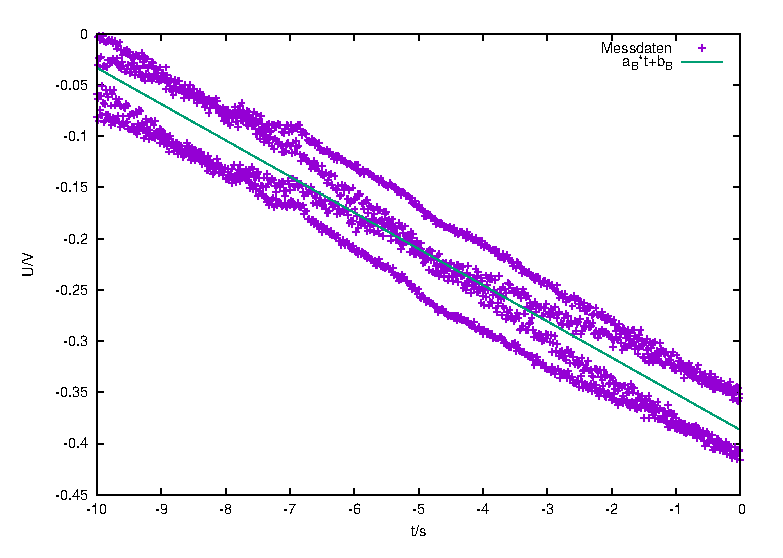
\includegraphics[width=\textwidth]{graphics/fit_Eingangsruhestrom_OVB084.eps}
    \caption{Spannungsverlauf zur Ermittlung des Eingangsruhestroms am
    OV B084, $C=1.5~\mathrm{nF}$}
    \label{fig:ERS_B}
\end{figure}
\begin{figure}[!ht]
    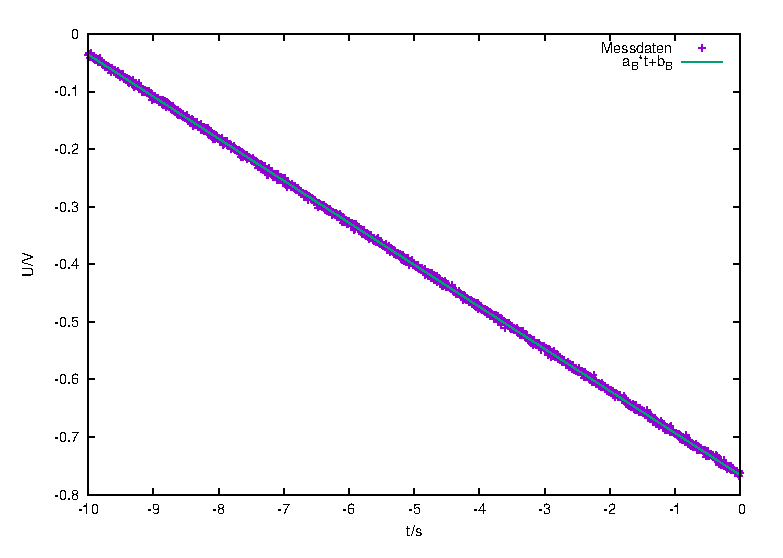
\includegraphics[width=\textwidth]{graphics/fit_Eingangsruhestrom_A109.eps}
    \caption{Spannungsverlauf zur Ermittlung des Eingangsruhestroms am A109,
    $C=4~\mathrm{\mu F}$}
    \label{fig:ERS_A}
\end{figure}

Die dort eingezeichneten Fit-Geraden ergeben jeweils einen Anstieg,
der es ermöglicht, den Strom zu berechnen.
Zur Beurteilung des Fehlers wird für die Kapazitäten ein
recht hoher Rundungsfehler von einer halben Stelle nach Angabe angenommen.

\begin{align*}
    a_B \,&=\, \left(-0.03537\pm 0.00024\right)~\mathrm{\frac{V}{s}}\\
          &=\, -0.03537 \, \left(1\pm0.66\%\right)~\mathrm{\frac{V}{s}}\\
    b_B \,&=\, \left(-0.3868 \pm 0.0014\right)~\mathrm V\\
          &=\, -0.3868 \, \left(1\pm 0.35\%\right)~\mathrm V\\
    C_B \,&=\,1.5~\mathrm{nF}\\
    \Rightarrow
    I_B \,&=\, \left(-53.1\pm2.2\right)~\mathrm{pA}\\
    &=\, -53.1\,\left(1\pm3.99\%\right)~\mathrm{pA}
\end{align*}

\begin{align*}
    a_A \,&=\, \left(-0.073033\pm 0.000020\right)~\mathrm{\frac{V}{s}}\\
          &=\, -0.073033 \, \left(1\pm0.03\%\right)~\mathrm{\frac{V}{s}}\\
    b_A \,&=\, \left(-0.76603 \pm 0.00012\right)~\mathrm V\\
          &=\, -0.76603 \, \left(1\pm 0.02\%\right)~\mathrm V\\
    C_A \,&=\,4~\mathrm{\mu F}\\
    \Rightarrow
    I_A \,&=\, \left(-290\pm40\right)~\mathrm{nA}\\
    &=\, -290\,\left(1\pm12.53\%\right)~\mathrm{nA}
\end{align*}

\subsubsection {Leerlaufverstärkung}

Die Leerlaufverstärkung wurde am \emph{OV B084, OV5} gemessen.
Als Widerstände wurde gewählt:

\begin{align*}
    R_g\,&=\,100~\mathrm{k\Omega}\\
    R_1\,&=\,10~\mathrm{k\Omega}\\
    R_2\,&=\,10~\mathrm{k\Omega}\\
    R_3\,&=\,100~\mathrm{\Omega}
\end{align*}

Die Messwerte sind in Tabelle \ref{tab:Leerlaufverst} protokolliert
und in Abbildung \ref{fig:Leerlaufverst} visualisiert.
Dabei wurde $U_a$ invertiert,
sodass die Phasenverschiebung $\phi$ nicht durch die Inversion des
Verstärkers beeinflusst wird.
Alle Spannungen sind Effektivwerte

\begin{table}[!ht]
    \centering
    \caption{Messwerte für Spannungen und Phasenverschiebung zur
    Bestimmung der Leerlaufverstärkung}
    \label{tab:Leerlaufverst}
    \begin{tabular}{r|r|r|r|r|r}
        $\nu/\mathrm{Hz}$&$U_e/\mathrm{mV}$&$U_a/\mathrm V$&$U_1/\mathrm{mV}$&
        $\phi/^\circ$&$v_u/\mathrm{db\,V}$\\
        \hline
                1&  598.0&  5.945&  0.7&   -0.1&123.13\\
               10&  597.9&  5.944&  2.1&    1.4&113.59\\
              100&  598.1&  5.927& 19.5&    4.0&94.21\\
             1000&  599.1&  4.940&159.9&   34.0&74.33\\
            10000&  600.1&  0.883&281.0&   84.0&54.57\\
           100000&  601.0&  0.079&257.0&  100.0&34.26
    \end{tabular}
\end{table}

\begin{figure}[!ht]
    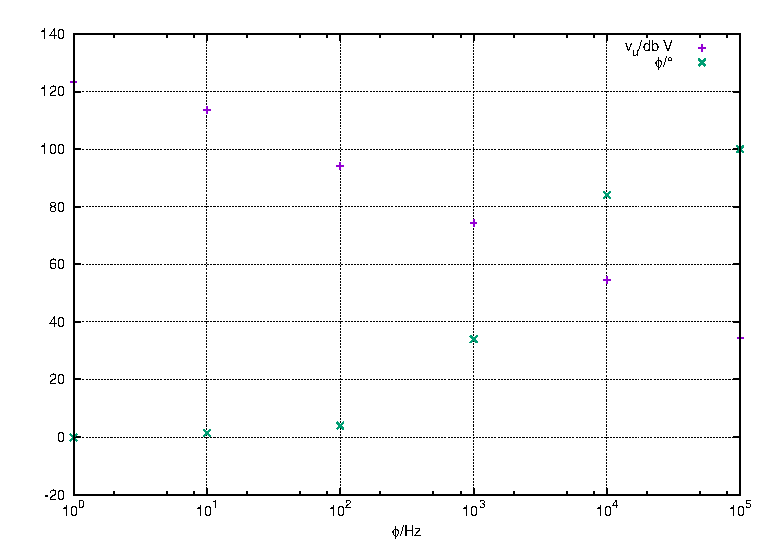
\includegraphics[width=\textwidth]{graphics/plot_leerlaufverst.eps}
    \caption{Leerlaufverstärkung $v_u$ und Phasenverschiebung $\phi$ in 
        Abhängigkeit von der angelegten Frequenz}
    \label{fig:Leerlaufverst}
\end{figure}

\pagebreak
\subsection {Grundschaltungen}

\subsubsection {Invertierender Verstärker}

Für den Aufbau eines invertierenden Verstärkers werden je ein Bild
vor, bei und über der oberen Grenzfrequenze aufgenommen.
Genutzt wird hierbei der Verstärker \emph{OV B084, OV5}.
Die Widerstände sind $R_e=10~\mathrm{k\Omega}$ und $R_g=100~\mathrm{k\Omega}$.
Die Bilder sind in Abbildung \ref{fig:InvVerst} dargestellt,
wichtige Größen in Tabelle \ref{tab:InvVerst} protokolliert.
Auch hier sind die Spannungen wieder Effektivwerte.
Die Granzfrequenz ist dann eingestellt,
wenn die Phasenverschiebung zwischen $U_e$ und dem invertierten $U_a$ gerade
$45^\circ$ beträgt.

Die theoretische Verstärkung beträgt
$v_{u,th}=-\frac{R_g}{R_e}=10=20~\mathrm{db\,V}$.

\begin{table}[!ht]
    \centering
    \caption{Messwerte am Invertierenden Verstärker}
    \label{tab:InvVerst}
    \begin{tabular}{r|r|r|r|r}
        $\nu$&$\phi/^\circ$&$U_e/\mathrm {mV}$&$U_a/\mathrm V$
        &$v_u/\mathrm{db\,V}$\\
        \hline
        $1~\mathrm{Hz}$&179.2&884&8.77&19.93\\
        $69~\mathrm{kHz}$&-135.6&888&6.25&16.95\\
        $1.6~\mathrm{MHz}$&-40&897&0.44&-6.19
    \end{tabular}
\end{table}

\begin{figure}[!ht]
    \centering
    \begin{subfigure}[t]{0.6\textwidth}
        \centering
        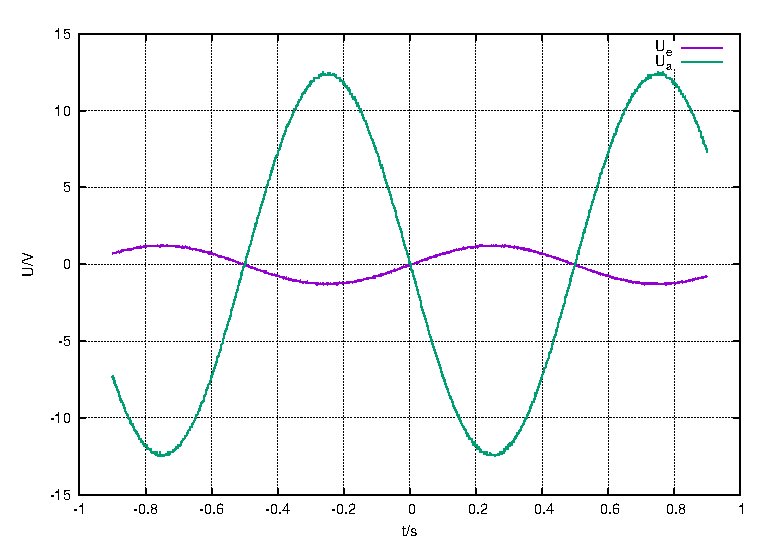
\includegraphics[width=\textwidth]{graphics/plot_invVers_u.eps}
        \caption{$\nu=1~\mathrm{Hz}$, $\phi=179.2^\circ$}
    \end{subfigure}

    \begin{subfigure}[t]{0.6\textwidth}
        \centering
        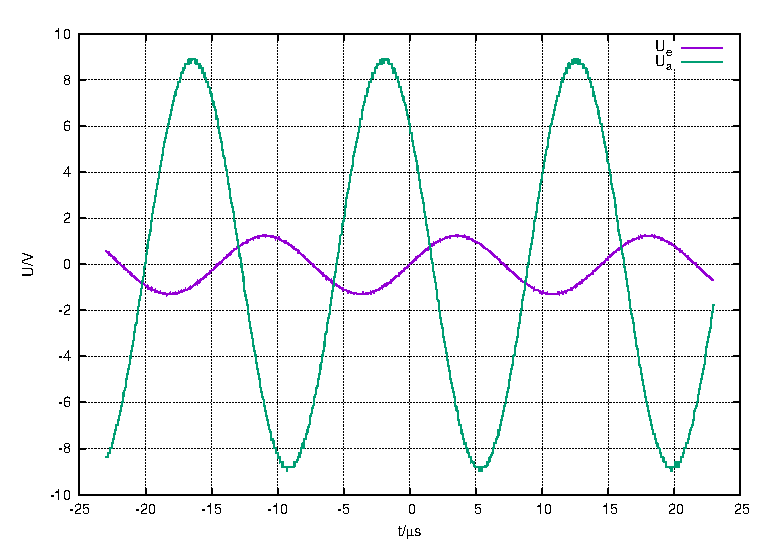
\includegraphics[width=\textwidth]{graphics/plot_invVers_g.eps}
        \caption{$\nu=69~\mathrm{kHz}$, $\phi=-135.6^\circ$}
    \end{subfigure}

    \begin{subfigure}[t]{0.6\textwidth}
        \centering
        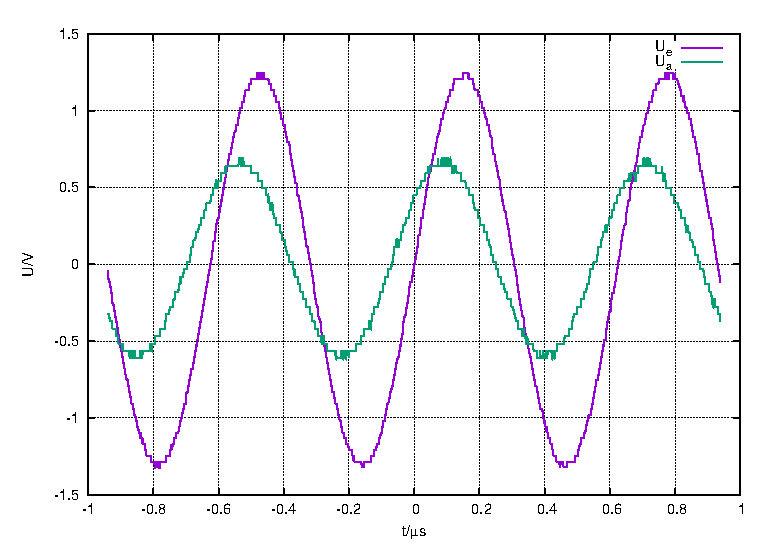
\includegraphics[width=\textwidth]{graphics/plot_invVers_o.eps}
        \caption{$\nu=1.6~\mathrm{MHz}$, $\phi=-40^\circ$}
    \end{subfigure}
    \caption{Verlauf von $U_e$ und $U_a$ am invertierenden Verstärker}
    \label{fig:InvVerst}
\end{figure}

\subsubsection {Nichtinvertierender Verstärker}

Der Nichtinvertierende Verstärker wird mit \emph{OV B084, OV5} so aufgebaut,
dass die theoretische Verstärkung
$v_{u,th}=3=9.52~\mathrm{db\,V}=1+\frac{R_g}{R_T}$
eingestellt ist.
Dazu werden die Widerstände $R_g=100~\mathrm{k\Omega}$ und
$R_T=50~\mathrm{k\Omega}$ gewählt zusammen mit der Frequenz
$\nu=21~\mathrm{kHz}$ gewählt,
die weit unterhalb der Grenzfrequenz liegt.
Es wird $U_e=1~\mathrm V$ als Effektivwert eines Rechtecksignals angelegt.

Gemessen wird ein Ausgangssignal mit $U_a=2.77~\mathrm V$.
Daraus resultiert eine reale Verstärkung von:

\begin{align*}
    v_u\,&=\,2.77\\
         &=\,8.85~\mathrm{db\,V}
\end{align*}

Zur Messung der Slew Rate wird der Anstieg des lieare Bereiches nach
Spannungsumpolung mittels Fit der Form $a_St+b_S$ ermittelt.
Hierbei ist $a_S$ die Slew Rate.
Dies ist in Abbildung \ref{fig:fit_slew} dargestellt.

\begin{figure}[!ht]
    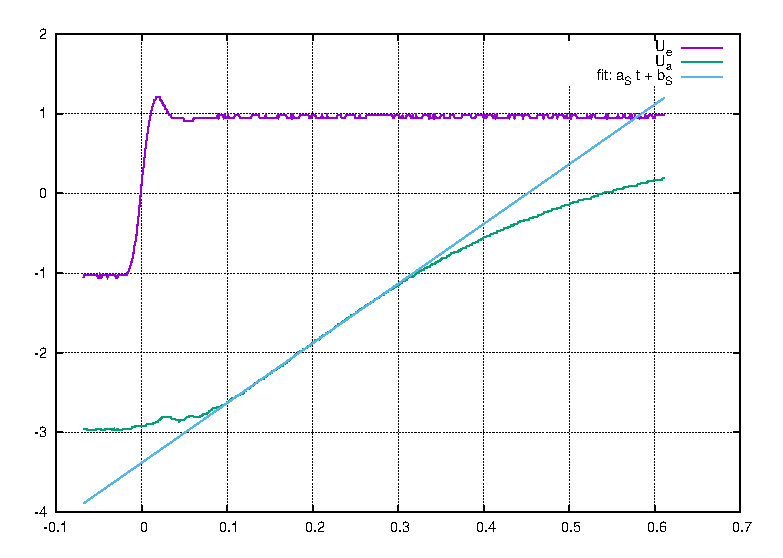
\includegraphics[width=\textwidth]{graphics/fit_slew_rate.eps}
    \caption{Fit zur Ermittlung der Slew Rate}
    \label{fig:fit_slew}
\end{figure}

Der Fit ergibt:

\begin{align*}
    a_S\,&=\,\left(7.494 \pm 0.012\right)~\mathrm{\frac{MV}{s}}\\
    &=\,7.494 \left(1\pm 0.15\%\right)~\mathrm{\frac{MV}{s}}\\
    b_S\,&=\,\left(-3.3814 \pm 0.0024\right)~\mathrm{V}\\
    &=\,-3.3814 \left(1\pm 0.07\%\right)~\mathrm{V}
\end{align*}

\pagebreak
\subsubsection {Stromspannungswandler und Schmitt-Trigger}

Für den Stromspannungswandler wird der Operationsverstärker \emph{OV B084, OV5}
verwendet,
für den Schmitt-Trigger \emph{OV B084, OV6}.
Die Widerstände sind $R_g=1~\mathrm{M\Omega}$, $R_e=10~\mathrm{k\Omega}$,
$R_1=50~\Omega$ und $R_2=600~\Omega$.

An $U_{a1}$ wird am Stromspannungswandler ein Signal mit positivem
Gleichspannungsteil gemessen,
das mit der Frequenz $\nu=100~\mathrm{Hz}$ entfernt an eine Sinusform erinnert,
siehe Abbildung \ref{fig:SSWandler_Ua1}.
Die Form des Signal kommt daher,
dass die Photodiode mit einer Leuchtstofflampe bestrahlt wird,
die mit Netzspannung $220~\mathrm V/50~\mathrm{Hz}$ betrieben wird.
Da die Stromrichtung für die Gasentladung egal ist,
entsteht ein Signal der Form $\sin^2(t)\propto\cos(2t)$,
sodass die Periodendauer $2\cdot50~\mathrm{Hz}$ zustande kommt.
Hinzu kommt ein Gleichspannungsteil durch die fluoreszente
Leuchtstoffbeschichtung.

\begin{figure}[!ht]
    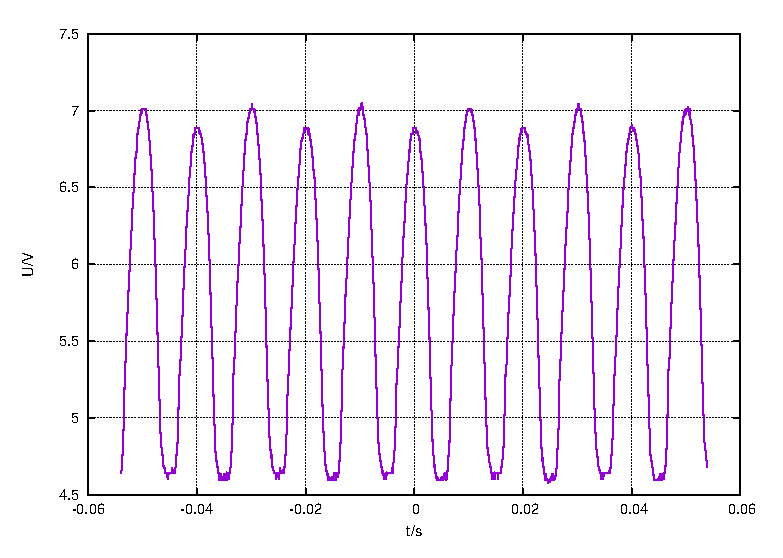
\includegraphics[width=\textwidth]{graphics/plot_SSW_Ua1.eps}
    \caption{$U_{a1}$ am Stromspannungswandler}
    \label{fig:SSWandler_Ua1}
\end{figure}

Für die Spannung am Stromspannungswandler wird als Gleichspannungsteil
etwa $U_{a1}=5.9~\mathrm{V}$ gemessen.
Folglich wird als $U_{ref}$ ein Wert in der Nähe gewählt,
$U_{ref}=5.55~\mathrm{V}$.
Die Signale am Schmitt-Trigger sind in Abbildung \ref{fig:plot_schmitt}
bei unterschiedlichen Beleuchtungen aufgetragen.
Abbildung \ref{fig:schmitt} zeigt den Verlauf von $U_{a2}$ in Abhängigkeit
von $U_{a1}$.

\begin{figure}[!ht]
    \begin{subfigure}{0.5\textwidth}
        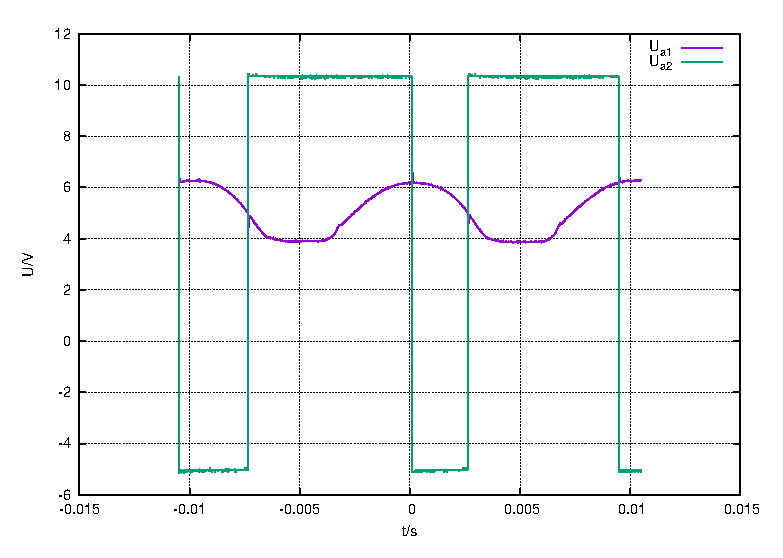
\includegraphics[width=\textwidth]{graphics/plot_SSW_low.eps}
        \caption{geringe Beleuchtung}
    \end{subfigure}
    \begin{subfigure}{0.5\textwidth}
        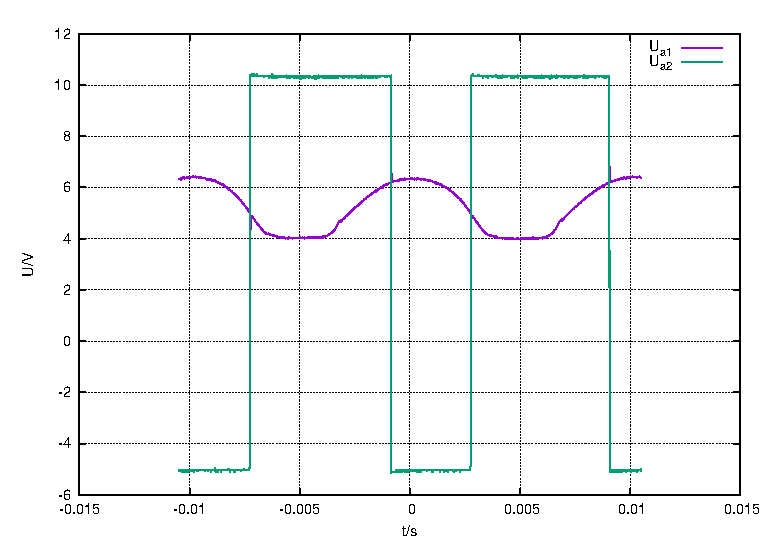
\includegraphics[width=\textwidth]{graphics/plot_SSW_high.eps}
        \caption{hohe Beleuchtung}
    \end{subfigure}
    \caption{$U_{a1}$ und $U_{a2}$ am Schmitt-Trigger}
    \label{fig:plot_schmitt}
\end{figure}

\begin{figure}[!ht]
    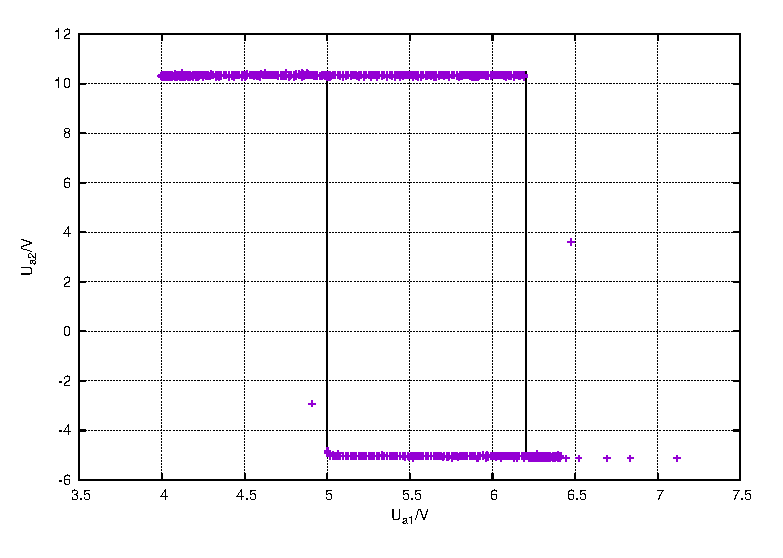
\includegraphics[width=\textwidth]{graphics/schmitt.eps}
    \caption{$U_{a2}$ in Abhängigkeit von $U_{a1}$ am Schmitt-Trigger}
    \label{fig:schmitt}
\end{figure}

Die Hysterese $\Delta U_S$ wurde mit dem Oszilloskop ausgemessen.

\begin{equation}
    \Delta U_S\,=\,1.32~\mathrm V
\end{equation}

\pagebreak
\section {Auswertung}

\subsection {Eigenschaften von Operationsverstärkern}

Als Offsetspannung für den Operationsverstärker \emph{OV B084, OV1}
wurde gemessen:

\begin{equation*}
    U_0\,=\,27~\mathrm{\mu V}
\end{equation*}

Dies liegt in der erwarteten Größenordnung von $~10^2~\mathrm{\mu V}$.

Für die Eingangsruheströme am \emph{OV B084, OV1} und \emph{A109}
wurde gefunden:

\begin{align*}
    a_B\,&=\,53.1~\mathrm{pA}\\
    a_A\,&=\,290~\mathrm{pA}
\end{align*}

Diese Werte liegen im Bereich $\mathrm{pA}$,
wenn auch etwas höher als erwartet.

FÜr Leerlaufverstärkung und Phasenverschiebung am \emph{OV B084, OV5}
wurden die Werte in Tabelle \ref{tab:Leerlaufverst} gefunden.
Bis zu $\nu=100~\mathrm{Hz}$ liegen die Werte für die Verstärkung
in der erwarteten Größenordnung $100~\mathrm{db\,V}$
und die Phasenverschiebung liegt bei nahe den erwarteten $0^\circ$.
Bei höheren Frequenzen nimmt die Verstärkung erwartungsgemäß ab,
die Phasenverschiebung zu.
Die Grenzfrequenz liegt hier etwas über $1~\mathrm{kHz}$.
Es konnte aufgrund der Messungenauigkeit des Voltmeters nicht mehr in Bereichen
nahe der Resonanz gemessen werden.

\subsection {Verstärker}

Für invertierenden und nichtinvertierenden Verstärker wurde der
Operationsverstärker \emph{OV B084} genutzt.

Für den invertierenden Operationsverstärker mit theoretischer Verstärkung
$v_{u,th}=20~\mathrm{db\,V}$ wurde eine reelle Verstärkung von
$\boxed{v_u=19.93~\mathrm{db\,V}}$ gefunden.
Diese liegt sehr nah am theoretischen Wert,
nimmt aber zur Grenzfrequenz wie erwartet ab bis zum Wert
$\boxed{v_{u,g}=16.95~\mathrm{db\,V}}$ bei einer Grenzfrequenz von
$\boxed{69~\mathrm{kHz}}$.
Weit oberhalt der Grenzfrequenz bei $1.6~\mathrm{MHz}$ wurde nur noch eine
Verstärkung von $-6.19~\mathrm{db\,V}$ gefunden,
das Ausgangssignal ist also sehr viel geringer als das Eingangssignal.
Der Verstärker sollte also nicht über $69~\mathrm{kHz}$ betrieben werden.

Bei einem nichtinvertierenden Verstärker mit theoretischer Verstärkung von
$v_{u,th}=9.52~\mathrm{db\,V}$ liegt die reelle Verstärkung nur noch bei
$\boxed{v_u=8.85~\mathrm{db\,V}}$.
Als Slew Rate wurde $\boxed{a_S=7.5~\mathrm{\frac{MV}{s}}}$ gefunden.
Bei einem idealen Verstärker wäre dieser Wert unendlich hoch,
doch ein endlicher Wert zeigt eine weitere weitere Frequenzbegrenzung für
hohe Spannungen auf.
Die maximale Frequenz bezüglich der Slew Rate in Abhängigkeit vom
Peak-to-Peak-Wert von $U_e$ ist gegeben durch:

\begin{equation*}
    \nu_{max}(U_e)\,=\,\frac{a_S}{v_u\,U_e}
\end{equation*}

Bei den angelegten $1~\mathrm V$ Effektivwert läge die maximale Frequenz
bezüglich der Slew Rate bei $\nu_{max}=1.9~\mathrm{MHz}$,
was weit über der Grenzfrequenz liegt und daher keine Bedeutung hat.
Für $U_e=1000~\mathrm V$ läge die Höchstfrequenz jedoch schon bei
$\nu_{max}=1.9~\mathrm{kHz}$,
sodass man für Hochspannungsanwendungen andere Lösungen suchen muss.

\subsection {Stromspannungswandler und Schmitt-Trigger}

Der Stromspannungswandler arbeitet wie erwartet und gibt den
Strom an der Diode als verstärkten Spannungswert aus.
Aus dem gefundenen Gleichspannungsteil ergibt sich:

\begin{align*}
    U_{a1}\,&=\,5.9~\mathrm V\\
    R_G\,&=\,1~\mathrm{M\Omega}\\
    \alignedbox{I_{FD}\,}{=\,5.9\mathrm{\mu A}}
\end{align*}

Dieser Strom liegt in einer erwarteten Größenordnung für eine Photodiode.

Abbildung \ref{fig:schmitt} zeigt das Verhalten des Schmitt-Triggers sehr gut.
Innerhalb der Hysterese, also zwischen $U_{S1}$ und $U_{S2}$ sind sowohl
Spannungen messbar, die binär 0 entsprechen, als auch Spannungen, die binär 1
entsprechen.
Unterhalb von $U_{S1}$ ist nur binär 1 vertreten und oberhalb von
$U_{S2}$ ist nur binär 0 vertreten.
Der Grund dafür ist, wie man in Abbildung \ref{fig:plot_schmitt} sieht,
dass im Zustand binär 0 solange verweilt,
bis das Signal $U_{a1}$ den Wert $U_{S1}$ unterschreitet.
Dort bleibt der Zustand binär 1 solange erhalten,
bis das Signal $U_{a1}$ den Wert $U_{S2}$ überschreitet.
Unterhalb dieses Wertes kann sich das Signal beliebig verhalten,
ohne eine Zustandsänderung in $U_{a2}$ zu erzeugen
und gleiches gilt umgekehrt für den Zustand binär 0.

\pagebreak
% \section {Quellen}
% \begin{thebibliography}{999}
% \bibitem {WalterHerms} G. Walter und G. Herms, Einführung in die Behandlung von Messfehlern -- Ein Leitfaden für das Praktikum der Physik, Universität Rostock 2006d
% \end{thebibliography}

\section* {Anhang}


\end{document}
%sagemathcloud={"zoom_width":100}
